%%%%%%%%%%%%%%%%%%%%%%%%%%%%%%%%%%%%%%%%%
% a0poster Portrait Poster
% LaTeX Template
% Version 1.0 (22/06/13)
%
% The a0poster class was created by:
% Gerlinde Kettl and Matthias Weiser (tex@kettl.de)
% 
% This template has been downloaded from:
% http://www.LaTeXTemplates.com
%
% License:
% CC BY-NC-SA 3.0 (http://creativecommons.org/licenses/by-nc-sa/3.0/)
%
%%%%%%%%%%%%%%%%%%%%%%%%%%%%%%%%%%%%%%%%%

%----------------------------------------------------------------------------------------
%	PACKAGES AND OTHER DOCUMENT CONFIGURATIONS
%----------------------------------------------------------------------------------------

\documentclass[a0,landscape,spanish,20pt]{a0poster}

\newcommand{\anchoFigura}{0.48}
\newcommand{\anchoFiguraPareto}{0.75}
% Include the helvet package
\usepackage{helvet}

% Set the default font to be palatino
\renewcommand{\sfdefault}{ppl}
%\usepackage[]{algorithm}
\usepackage{algpseudocode}
%S\usepackage[spanish, mexico]{babel}
%\selectlanguage{spanish}
\usepackage[utf8]{inputenc}
%\usepackage{float}
\usepackage{mathrsfs}
\usepackage{amsmath}
\usepackage{ragged2e}
\usepackage{multicol} % This is so we can have multiple columns of text side-by-side
\columnsep=100pt % This is the amount of white space between the columns in the poster
\columnseprule=3pt % This is the thickness of the black line between the columns in the poster
\usepackage{vwcol}  
\usepackage[svgnames]{xcolor} % Specify colors by their 'svgnames', for a full list of all colors available see here: http://www.latextemplates.com/svgnames-colors

%\usepackage{times} % Use the times font
\usepackage{palatino} % Uncomment to use the Palatino font

\usepackage{graphicx} % Required for including images
\graphicspath{{figures/}} % Location of the graphics files
\usepackage{booktabs} % Top and bottom rules for table
\usepackage[font=Large,labelfont=bf]{caption} % Required for specifying captions to tables and figures
\usepackage{amsfonts, amsmath, amsthm, amssymb} % For math fonts, symbols and environments
\usepackage{wrapfig} % Allows wrapping text around tables and figures

\usepackage{titlesec}
\usepackage{framed}
\usepackage[Large,bf, raggedright]{subfigure} % subfiguras
\usepackage{subfig}
\usepackage{floatrow}
\usepackage{pgfplots}
\usepackage[eulergreek]{sansmath}
\pgfplotsset{compat=1.3, width=70mm, height=60mm}
\pgfplotsset{
tick label style = {font=\sansmath\sffamily},
every axis label = {font=\sansmath\sffamily},
legend style = {font=\sansmath\sffamily},
label style = {font=\sansmath\sffamily}
}

\titlespacing*{\section}{0pt}{10pt}{0pt}
\definecolor{shadecolor}{rgb}{0.196078431,0.278431373,0.462745098}
\newcommand*{\bigH}{\scalebox{1.5}{\ensuremath{\mathscr{H}}}}

\begin{document}

%----------------------------------------------------------------------------------------
%	POSTER HEADER 
%----------------------------------------------------------------------------------------

% The header is divided into two boxes:
% The first is 75% wide and houses the title, subtitle, names, university/organization and contact information
% The second is 25% wide and houses a logo for your university/organization or a photo of you
% The widths of these boxes can be easily edited to accommodate your content as you see fit
 
\begin{minipage}[b]{1\linewidth}
\begin{minipage}{0.08\linewidth}
\includegraphics[width=1\columnwidth]{figures/photo.jpg}
\end{minipage}
\begin{minipage}{0.8\linewidth}
\begin{shaded}
\centering
\Huge \color{White} \fontfamily{phv} \textbf{Multi-objective optimization based on parameter tuning of CLAHE to achieve different contrast levels in medical images}\\ [0.5cm]% Title
                                             \Large \textbf{Luis G. Moré, Marcos Brizuela, José L. Vázquez, Diego Pinto, Horacio Legal, } 
\Large \textit{Facultad Politécnica - Universidad Nacional de Asunción}
\end{shaded}
\end{minipage}
\begin{minipage}{0.08\linewidth}
\centering
\includegraphics[width=1\columnwidth]{figures/qrcode.jpg}
\end{minipage}


\end{minipage}

\line(1,0){3100}

%
%\begin{minipage}[b]{0.25\linewidth}
%\includegraphics[width=19cm]{photo.jpg}\\
%\end{minipage}

%\vspace{0.5cm} % A bit of extra whitespace between the header and poster content

%----------------------------------------------------------------------------------------

\begin{multicols}{3} % This is how many columns your poster will be broken into, a portrait poster is generally split into 2 columns


%----------------------------------------------------------------------------------------
%	INTRODUCTION
%----------------------------------------------------------------------------------------

%\color{SaddleBrown} % SaddleBrown color for the introduction

\section*{ \begin{shaded} \color{White} \huge \centering Introduction \end{shaded}}



{ \Large 

\color{Black}

Contrast of medical images show particular contrast features, because there might be notorious contrast differences because of the attenuation characteristics of X-Rays. 

Local improvement approaches prove to be extremely useful when enhancing details in medical images. In our proposal a meta-heuristic for optimization will be used, in order to tune input parameters of the contrast enhancement algorithm. \medskip

\textbf{Objective: }Obtain images with different relationships between contrast and distortion, in order to highlight different features, which is useful for analysis performed by the specialist. 



}

\color{Black} % DarkSlateGray color for the rest of the content

\section*{ \begin{shaded} \color{White} \huge \centering Method \end{shaded}}

{ \Large
\color{Black}

\begin{wrapfigure}{r}{0.6\linewidth}
\vspace{-1pt}
\hspace{-1pt}
\centering
\includegraphics[{width=\linewidth}]{figures/particula_clahe3.png}
\caption{ \Large Interaction among $CLAHE$, $MOPSO$ particle and objective functions evaluation.}
\label{fig:particula_clahe}
\end{wrapfigure}

The Figure \ref{fig:particula_clahe} shows how Multi-objective PSO-CLAHE ($MOPSO-CLAHE$) based on $SMPSO$ is implemented to tune the parameters of CLAHE. The resulting images are automatically evaluated according to the metrics $Entropy$ ($\bigH$) and $SSIM$, and the best results measured by these shape a Pareto set for the image being processed. 

}

\section*{ \begin{shaded} \color{White} \huge \centering Results \end{shaded}}

%----------------------------------------------------------------------------------------
%   MATERIALS AND METHODS
%----------------------------------------------------------------------------------------
\color{Black} % DarkSlateGray color for the rest of the content

{ \Large

\begin{itemize}

\item For every selected test image (http://openi.nlm.nih.gov/), 30 executions of $MOPSO-CLAHE$ were performed, with populations composed by 100 particles, and 100 iterations for every execution. Every particle (potential solution) is automatically evaluated by $MOPSO-CLAHE$ according to the metrics adopted.
\item Approximately 300 non-dominated solutions were obtained for every image.
\item Every non-dominated solution is an image with different compromise between \textit{Entropy} and \textit{SSIM}, as it can be seen in Figure \ref{fig:resultado_chest}(c) and Figure \ref{fig:resultado_mammogram}(c).
\item Fine details of images are preserved, as in Figure \ref{fig:resultado_mammogram}(b), \ref{fig:resultado_mammogram}(c)  and main characteristics are highlighted, as in Figure \ref{fig:resultado_chest}(b). 
%\item The pareto sets for those images are shown in Figure \ref{fig:resultado_mammogram} and Figure \ref{fig:resultado_chest}.

\end{itemize}

}

\begin{figure}[H]
\centering
\subfigure[]{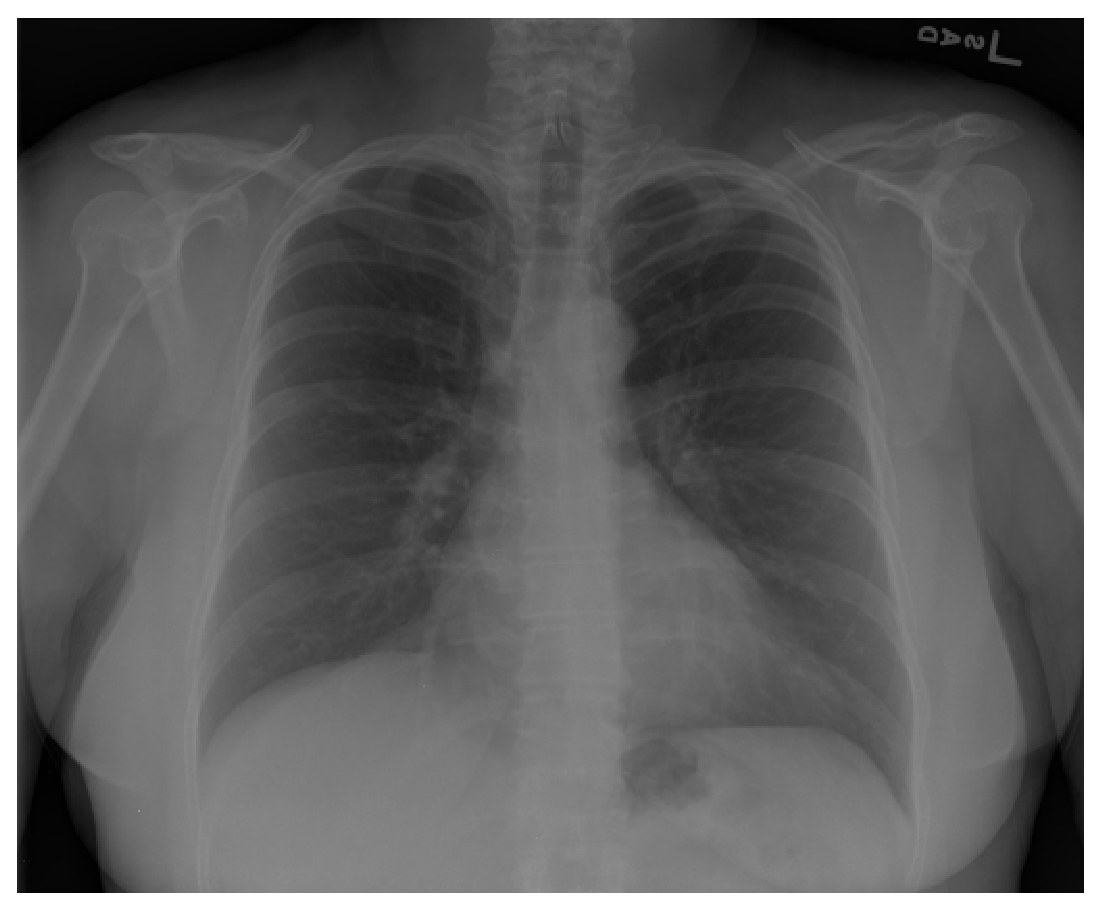
\includegraphics[width=0.48\columnwidth]{figures/100_IM-0002-1001.eps}}
\hspace{1pt}
\subfigure[]{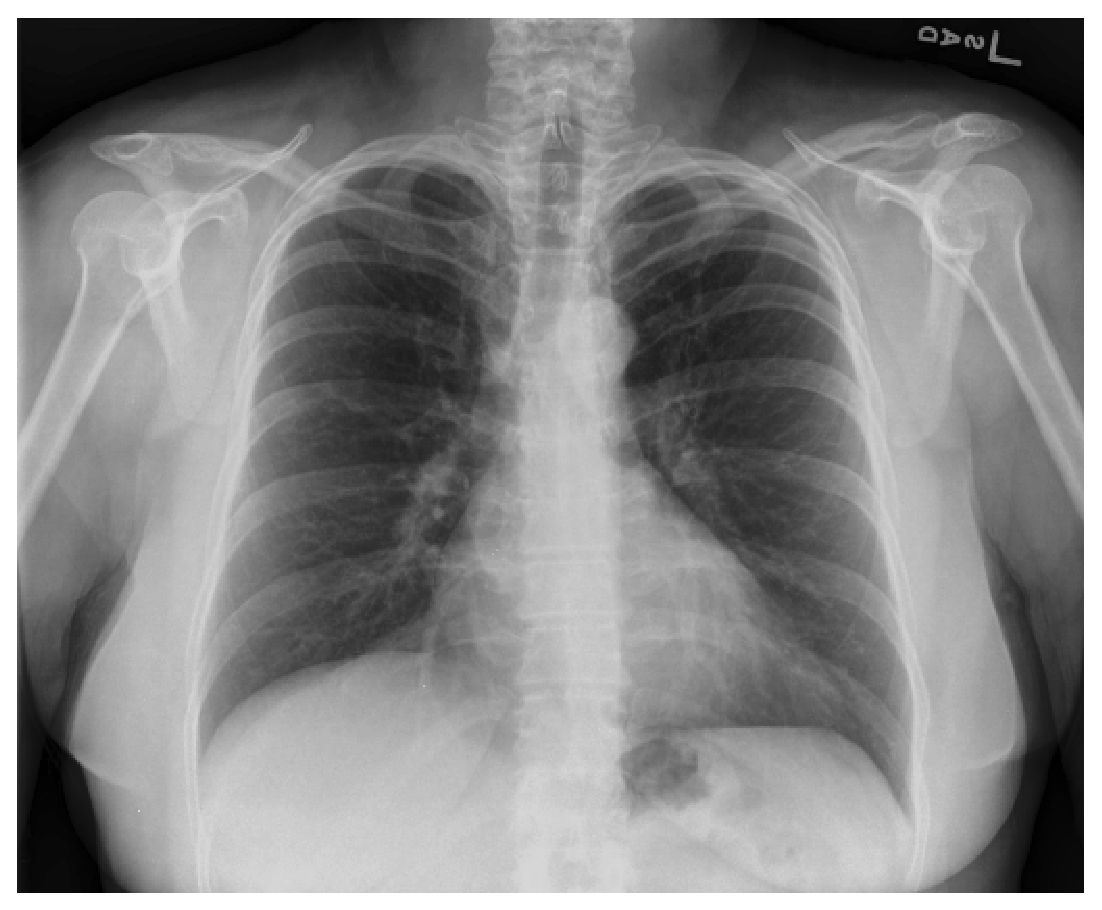
\includegraphics[width=0.48\columnwidth]{figures/1182-100_IM-0002-1001.eps}} \\[5pt]

\subfigure[]{

\pgfplotsset{every axis/.append style={
thick,
tick style={semithick}}}
\begin{tikzpicture}
\begin{axis}[height=12cm, width=0.95\columnwidth, xlabel={Entropy}, ylabel={SSIM},domain = 0:1, xtick={0.85, 0.87, 0.90,0.93,0.95,0.97, 0.985,1.0},
ytick={0.0,0.2,0.4,0.6,0.8,1.0}]
\addplot+[
only marks,
scatter,
mark=halfcircle*,
mark size=2.9pt]
table[meta=label]
{scattered_example.dat};
\end{axis}
\end{tikzpicture}


}


\caption{(a) Original Image. $SSIM$=1.0  \protect\bigH=0.8536 (b) Resultant image. $SSIM$=0.9688 \protect\bigH=0.7922 (c) Pareto set related to this image.}
\label{fig:resultado_chest}
\end{figure}

\begin{figure}[H]
\subfigure[]{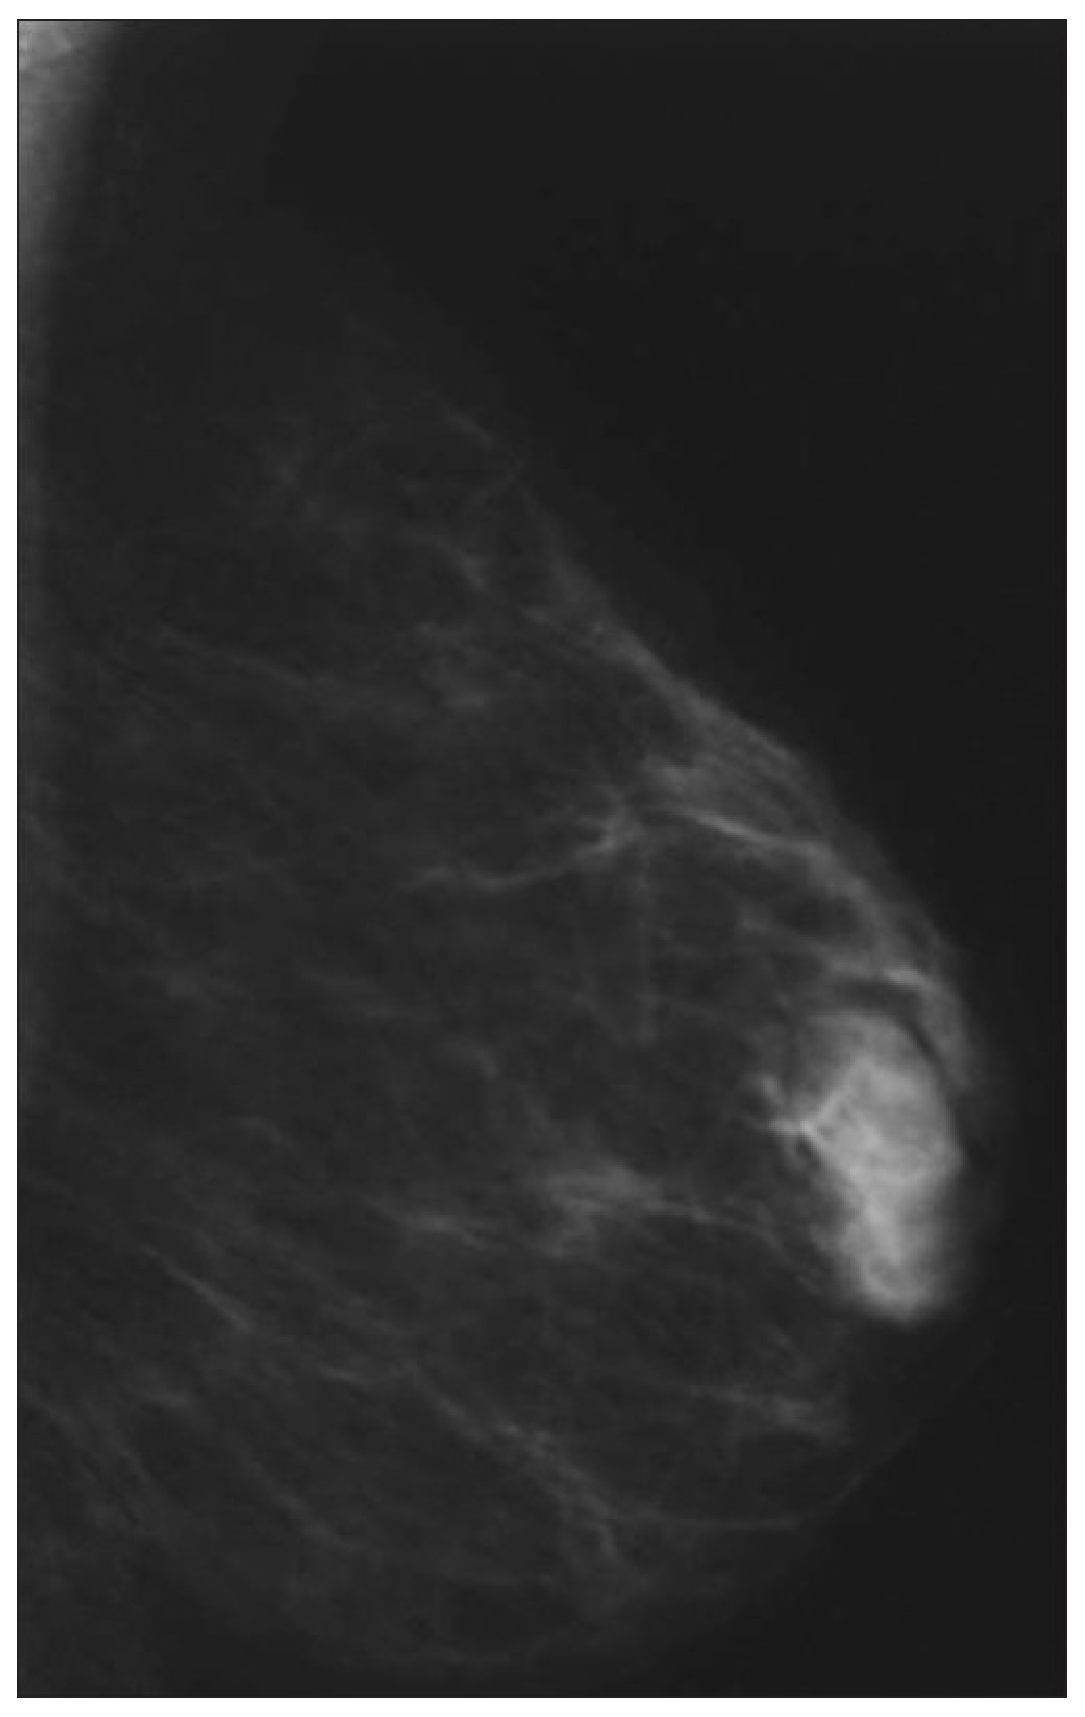
\includegraphics[width=0.3\columnwidth]{figures/3715982_IJMPO-34-47-g001.eps}}
\hspace{1pt}
\subfigure[]{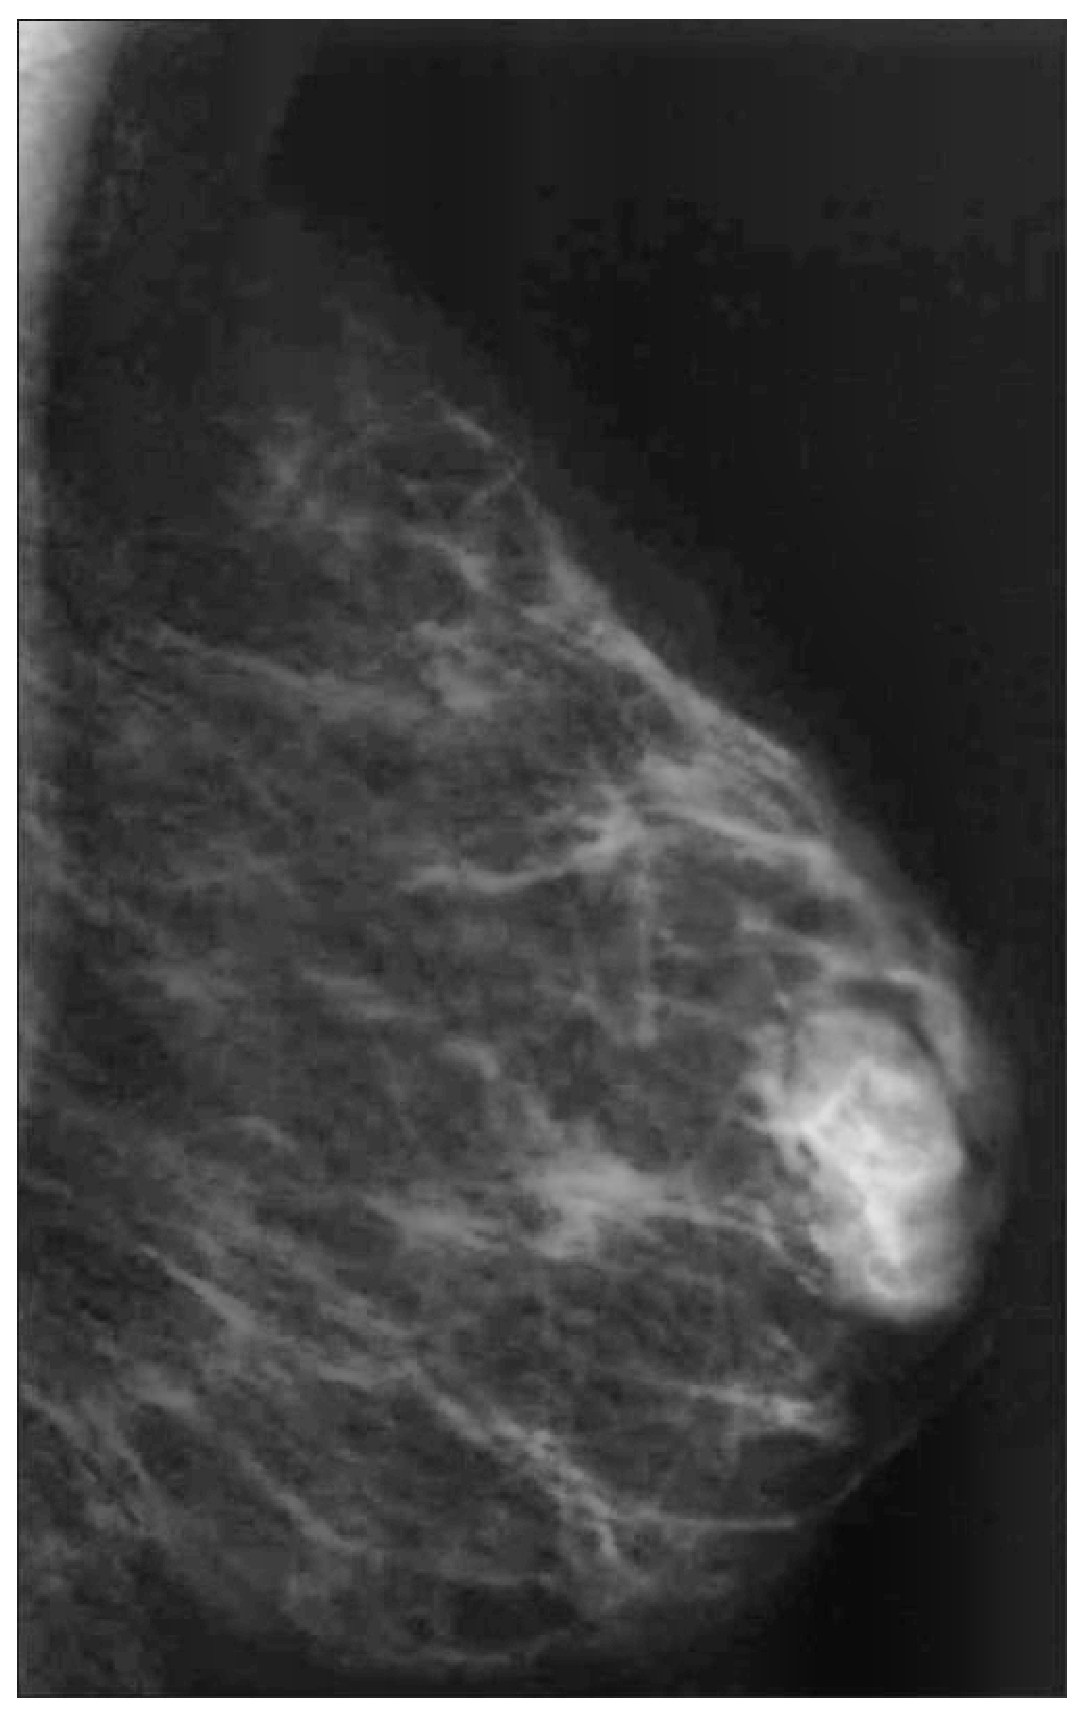
\includegraphics[width=0.3\columnwidth]{figures/11608-3715982_IJMPO-34-47-g001.eps}}
\hspace{1pt}
\subfigure[]{\includegraphics[width=0.3\columnwidth]{figures/11487-3715982_IJMPO-34-47-g001.png}}


\subfigure[]{

\pgfplotsset{every axis/.append style={
thick,
tick style={semithick}}}
\begin{tikzpicture}
\begin{axis}[height=12cm, width=0.95\columnwidth, xlabel={Entropy}, ylabel={SSIM},domain = 0:1, xtick={0.60,0.70,0.80,0.85,0.90,0.95,1.0},
ytick={0.0,0.2,0.4,0.6,0.8,1.0}]
\addplot+[
only marks,
scatter,
mark=halfcircle*,
mark size=2.9pt]
table[meta=label]
{scattered_chest.dat};
\end{axis}
\end{tikzpicture}

}

\caption{ (a) Mammography. $SSIM$=1.0 \protect\bigH=0.6235 (b) Resultant image. $SSIM$=0.8032 \protect\bigH=0.8549 (c) Resultant image. $SSIM$=0.6121 \protect\bigH=0.91393 (d) Pareto set related to this image.}
\label{fig:resultado_mammogram}
\end{figure}

%------------------------------------------------


\color{DarkSlateGray} % Set the color back to DarkSlateGray for the rest of the content


\section*{\begin{shaded} \color{White} \huge \centering Conclusions \end{shaded}}

{
\Large
\begin{itemize} \justifying
\item $MOPSO-CLAHE$ approach is successful at contrast enhancement, by tuning $CLAHE$ input parameters, and evaluating $Entropy$ (contrast) and $SSIM$ (Image quality assessment) simultaneously.
\item The pareto sets show a compromise between $Entropy$  and $SSIM$  in terms of maximization, which indicates that both metrics are complementary.
\item \textbf{Future work:} Test optimization-based contrast enhancement using new metaheuristics, IQA metrics, and public image databases. Establish new compromises between metrics, analytically and using pareto sets.
\end{itemize} 

}

%\section*{\begin{shaded} \color{White} \huge \centering Acknowledgments and info \end{shaded}}
%\centering
%\frame{\includegraphics[width=0.21\columnwidth]{figures/photo.jpg}}
%\hspace{1pt}
%\frame{\includegraphics[width=0.21\columnwidth]{figures/qrcode.jpg}}

%----------------------------------------------------------------------------------------
%	CONCLUSIONS
%----------------------------------------------------------------------------------------


\end{multicols}
\end{document}